\chapter{Introduction} \label{ch:intro}

This document constitutes the present author's efforts to organize a body of literature concerning the development of: spatial music and instruments, spatial audio recording and reproduction tools, and XR frameworks, which can all be jointly used towards musical experimentation. The focus of this work is to use Free and Open Source Software (FOSS) and low-cost solutions which might allow for greater proliferation of spatial music. In this work we will talk about the history of pioneering composers of \textit{spatial music} as well as what FOSS exists today for the creation, documentation and dissemination of these works. The following list outlines the particulars of each chapter.

\begin{enumerate}

    \item \textbf{Chapter \ref{ch:intro}:} introduction to the science of spatial sound. This chapter talks about the psycho-acoustics of spatial sound and some basic principles of the auditory system related to 3D audio.
    \item \textbf{Chapter \ref{ch:spat-mus}:} creation of spatial music, specifically in a live context. We also discuss spatial instruments including: controllers, augmented instruments (traditional instruments enhanced via controllers), and spatial-synthesis tools\footnote{These are controllers which perform both synthesis and spatialization tasks simultaneously.}.
    \item \textbf{Chapter \ref{ch:spat-aud}:} capture and reproduction of these live experiences, with a focus on fixed-media tools. 
    \item \textbf{Chapter \ref{ch:xr-mus}:} alternative reproduction methods, specifically those involving Extended Reality (XR) tools and binaural synthesis.
    \item \textbf{Chapter \ref{ch:conclusion}:} discussion and summaries of previous chapters and an overview of the possible future of spatial music.
    
\end{enumerate}

In \textbf{Chapter \ref{ch:intro}} we will introduce the concept of spatial audio and focus primarily on the psycho-acoustic principles exploited in these works. We will also talk about the art, physics, and cognition of spatial audio. This chapter is meant to give some context to the later three chapters, which focus more on specific issues surrounding spatial audio. In particular the following three chapters are structured as follows:

Sometimes, although not always, spatial instruments are inextricably linked to a musical work, which is why we decided to use a \textbf{Chapter \ref{ch:spat-mus}} to cover both of these topics. In this chapter we focus on computer-music systems that one might employ for the generation of spatial music in a live context. This forms a contrast to chapter \ref{ch:spat-aud} in which we reiterate some of the technologies already mentioned, with a focus, however, on systems better suited for fixed-media works. 

\textbf{Chapter \ref{ch:spat-aud}}, in addition to discussing spatial audio reproduction using fixed-media tools, also discusses spatial audio recording. We cover the history of these techniques, continue with an overview of state-of-the-art systems, and finally discuss some open-source solutions for both of these problems. The goal here is to discuss how to record the live music experiences, and how to reproduce these recordings once they have been acquired. 

Finally, \textbf{Chapter \ref{ch:xr-mus}} discusses how contemporary extended reality (XR) systems can be exploited to enhance the musical experience of multi-channel music. Our main focus here is to present how XR can be used as a dissemination tool allowing the public greater access to this type of music. As a way to contrast the access issue surrounding XR, and in order to be thorough, we will also discuss some XR tools that are not as low-cost or open-source.

Each of these chapters has an associated proposal that connects with the material covered in the related chapters. These three proposals can be found in the appendix of this work. The chapters \ref{ch:intro} and  \ref{ch:conclusion} do not have associated proposals, since these are only contextual chapters. 
All of the figures in this body of work fall under the Creative Commons license. Any figures which do not have citation were created by the author and also fall under this designated category. We encourage the reader to use these figures for their own work. 

\todo[inline]{there are many different licenses. I have to go back and check what kind of licenses all these figures have. it would also be good to have an appendix that describes the different licenses for media and code since these are important to our work.}

\section{Physics of Sound}

%https://books.google.com.bo/books?id=OywDx9pxCMYC&pg=PA1&source=gbs_toc_r&hl=es-419#v=onepage&q&f=false

\section{Auditory System}

% https://commons.wikimedia.org/wiki/Ear#/media/File:Ear-anatomy.png

\section{Neurophysiology of Spatial Sound}
%http://cognet.mit.edu/book/auditory-neuroscience

\section{Art of Spatial Sound}

Space as a parameter of music-making is a feature which has been explored by composers for hundreds of years. Unfortunately, most musicians have a limited understanding of the possibilities that modern systems provide them and continue to operate on the basis of two-dimensional sound\footnote{Left/right panning plus distance modeled via amplitude changes or the addition of reverberation. A three-dimensional model would include height.}. Despite gargantuan efforts by the audio industry to expand commercial systems from stereo to more sophisticated formats, two-channel audio reproduction systems have remained the \textit{de facto} playback method in most homes due to their accessibility and simplicity. 

Before the rise of electro-acoustic composers, many artists experimented with space as a parameter of composition by including within their scores: the placement of musicians in different parts of the concert hall; choreographed trajectories for musicians; or using height by placing musicians in balconies. Many challenges that existed then remain now: synchronicity between players, architectural changes between venues, or, providing a consistent experience for all audience members regardless of their seat. 

Avant-garde composers in the 20th century pushed the envelope further by taking advantage of the technological developments of their era. With the advent of transmitted and recorded sound, \textit{disembodied sound} - a musicological term referring to the displacement in space-time of musician and sound - found a permanent role in the \textit{acousmatic}\footnote{Acousmatic generally means musical works where the musicians are not present. We only experience pre-recorded sounds in these types of works.} works of: Schaeffer, Xenakis, and Cage, to name a few. These acousmatic works, meant for reproduction over loudspeakers, made great use of spatial audio technologies such as the \textit{quadraphonic} or \textit{octophonic} sound systems\footnote{Four and eight channel sound systems, respectively.}, which were being developed at the time. 

Unfortunately, despite great scientific leaps, many of these older works cannot be fully appreciated by the general public since these high-end sound reproduction systems remain protected by privileged institutions. Commercial movie theatres, which harbor similar systems, have no financial incentive to reproduce these works. Part of the motivation of this thesis is to explore accessible techniques for the creation, documentation, and dissemination of works which employ spatial sound as a primary component of the compositional process. 

While many composers today, in well-funded Universities, have the pleasure to explore spatial sound through the use of multi-channel systems, much of their detailed work commonly gets \textit{down-mixed}\footnote{Compressed down from a multi-track format to stereo, usually for commercial purposes.} to stereo formats prior to distribution. If the spatial attributes of a particular sound are indeed important to the composition, this ultimate representation leaves much to be desired. Luckily, many free and open-source solutions exist for audio engineers to create and re-distribute works of this variety preserving the environmental auditory elements pertinent to the works. Our intention is to highlight some of the best low-cost solutions available, giving artists greater freedom in the music-making process.

In addition to discussing technologies available for the creation, recording, and presentation of 3D audio - in a musical context - we will discuss some of the technical challenges inherent in these productions. Namely, we will consider the difficulty of 3D sound reproduction based on computer: storage, speed, and changing operating systems (OS). We hope this work proves useful for any composer interested in the minutiae of the science, and art, of \textit{spatial music}.

\section{Psycho-acoustics of Spatial Sound}

Before we can understand the mathematical details behind different 3D audio technologies\footnote{3D audio is another name given to the field of spatial audio. In musical domain we often refer to this practice as sound \textit{diffusion}.}, we should discuss some of the psycho-acoustic principles on which all spatial audio technologies rely. Many authors have written extensively about the subject, with entire books having been dedicated to the subject - Blauert's 1997 \cite{blauert1997spatial} being perhaps the most popular. Here we will give only a short account of the many experiments that have been undertaken in this domain in order to inform the reader of some of the most salient features of the auditory system which inform our perception of sounds.

From the psycho-acoustic perspective, the most important feature of the auditory system is our ability to localize sound. This is perhaps why so much attention has been devoted to the subject in the psycho-acoustic community. Having a sensitive auditory localization system poses an evolutionary advantage; being able to detect the presence of a predator, before it can reach us, is likely why we have developed the ability to localize sound. Similarly, being able to detect prey, before it can escape, could be evolutionarily advantageous. 

A number of perceptual mechanisms work in conjunction, and amalgamate into a single sensory experience, informing our understanding of sound origins (directionally speaking). Not only are we conditioned to use acoustic cues to draw these conclusions, but memory and vision also form a part of this complex model \cite{kendall19953}. Our subconscious contains a mental map of the prevailing origin of different sounds based on prior experience which informs our predictions of source orientation and direction. 

For example: we seldom hear birds chirping below us because they generally fly above our heads, or rest on branches that are higher than us. As a result, you will seldom see a bird-watcher searching for a particular species below them. They can safely assume the sound they hear comes from above, even if they are not sure. Furthermore, if they momentarily perceive that same bird to indeed be below them, for whatever reason, they will likely confirm or refute this suspicion by looking in that direction, and adapt their prediction based on the confluence of sensory information. 

Our auditory model of sound localization is quite complex, especially for multiple sources in spaces. When sound waves travel through air, if there is more than a single source, the pressure waves constructively and destructively interfere, making position estimations harder. Additionally, if the space is very \textit{reverberant}, if there are many reflections from walls, such as in a chapel, these predictions might become even more complicated to make. Figure \ref{fig:cosine-wave} shows a depiction of a cosine wave advanced in time, modified to show nodes and antinodes. \textit{Constructive} and \textit{destructive interference} refers to two or more pressure waves' ability to increase or decrease in amplitude based on interactions with each other. For example, a negative pressure \textit{antinode} might perfectly cancel a positive pressure antinode when two waves of equal frequency are offset in phase by 180\textdegree.

\begin{figure}[ht!]%force figure here, top, strict
\centering
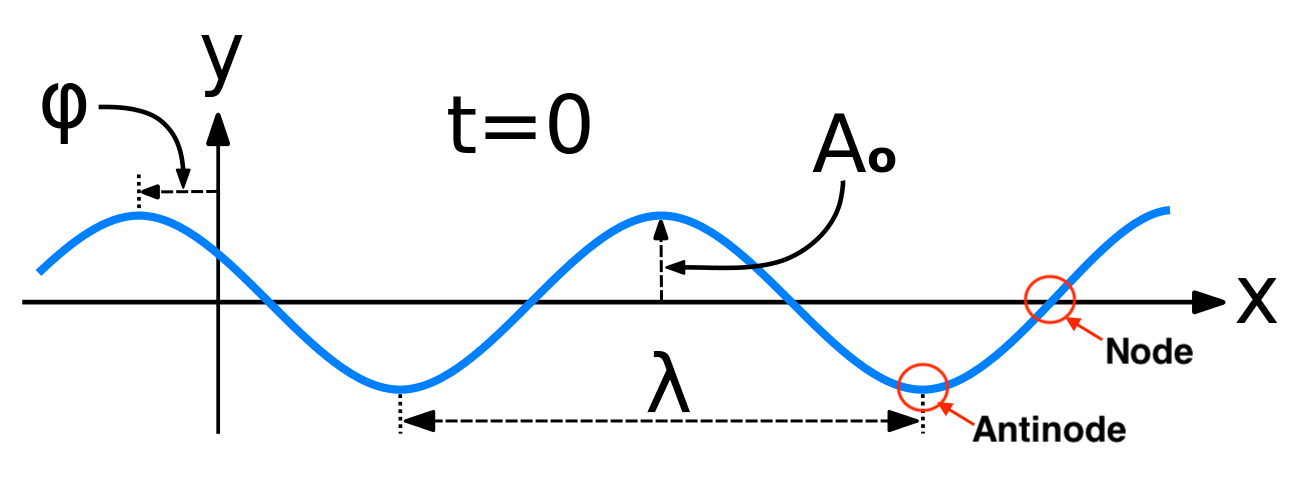
\includegraphics[width=0.8\textwidth]{img/cosine-wave.png} 
%\captionsetup{justification=centering}
\caption{Cosine Wave \cite{FileWave97:online}}
% attribution-share alike
\label{fig:cosine-wave}
\end{figure}

It is useful within this context to distinguish between source localization of \textit{near-field} and \textit{far-field} sources. As their names suggest, near-field sources are those that are proximal and far-field sources are those which are relatively distant from us. These definitions have real world implications, namely, near-field sources will arrive at our ears before any reflections muddle our perception of sound direction arrival. In contrast, far-field sources, in the real world, will produce complex spectra, since reflections and direct sound will interact in unpredictable ways. 

It is useful to further define two common conditions for sounds sources: those in \textit{free-fields} and those in \textit{diffuse-fields}. Free-field refers to an environment in which there is no reverberation; in other words, there are no surfaces upon which the sound may reflect. This condition is seldom found in nature, however, \textit{anechoic chambers}, rooms with no echoes, such as the one in Figure \ref{fig:ibm-anechoic}, have been designed specifically with this characteristic in order to conduct acoustic experiments. 

In contrast, diffuse-field refers to a condition in which prominent reflections are present, ideally with equal energy arriving from all directions. In architectural acoustics, diffusion will often be introduced intentionally, such as in concert halls, in order to spread energy evenly across the entire listening space. In between these two extremes there exists a continuum of acoustic spaces, each with their own acoustic characteristics, such as the: \textit{reverberation time} of the room, or the shortest reflection path from a source to a subject - whether that be a person or a receiver. 

\begin{figure}[ht!]%force figure here, top, strict
\centering
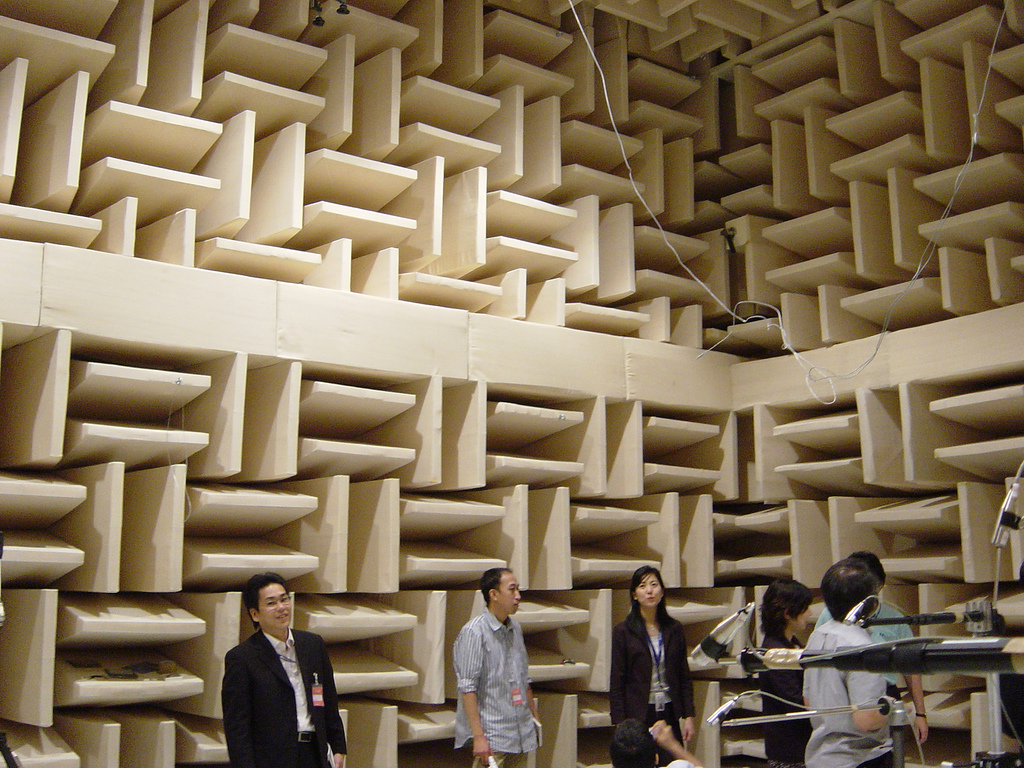
\includegraphics[width=0.6\textwidth]{img/ibm-anechoic.jpg} 
%\captionsetup{justification=centering}
\caption{IBM Anechoic Chamber \cite{FileIBMA4:online}}
\label{fig:ibm-anechoic}
\end{figure}

\todo[inline]{RT60, room acoustics, relevant to microphone calibration project. windowing. IR measurements. diffuse-field equalization. etc.}

\subsection{HRIRs}\label{subsec:hrirs}

An important aspect of spatialization in the musical domain, in addition to horizontal and vertical direction of sounds, is the distance of the event in relation to listener. For these three critical localization parameters\footnote{These being: horizontal position, vertical position, and distance.} various associated auditory mechanisms exist in the acoustic domain which facilitate our ability to place sources in space. 

In \textit{near-field} conditions, \textit{auralization} systems, systems that seek to replicate natural phenomena via digital means, tend to model distance as an independent characteristic of directional acoustic propagation. A common definition of near-field, albeit informal, is: anything within arms reach, or between 0.5m and 1m (\cite{Betbeder.2017})\footnote{1-2m is the typical distance for HRTF measurements.}. The idea behind this formal separation of near and far field is to exploit "tricks" in sound system design which help simulate real-world acoustic conditions at a much lower computational cost. By analyzing real-world acoustic snapshots, taken with microphones as \textit{impulse responses} (IR), we can observe that many acoustic spaces exhibit similar behaviors, statistically speaking, in particular regions of their IRs. By exploiting these similarities, it is possible to build systems which require less computational power while performing the same functions of more "expensive" algorithms.

Any acoustic space can be considered a linear time-invariant (LTI) system\footnote{LTI systems are a classification of engineering systems which can be fully described by an impulse response \cite{LinearTi32:online}.} which can be characterised by a single IR much like any digital or analog filter. Subtle changes in air pressure as a function of temperature can affect sound propagation, but for all intents and purposes this theory holds true. Inside the near-field, the abundance or lack of reverberant sound, caused by reflections from surfaces, can contribute to our perception of sound distance. However, it is more common to model the diffuse-field/far-field attributes independently, and use a complimentary system, based on free-field/near-field techniques, for horizontal and vertical auralization.

Within our free/near-field condition, we are not concerned with IRs of a single omni-directional acoustic sensor (for spatialization systems) but rather with the analysis of two impulse responses, ideally captured at the listeners ears. For this purpose there exist various methodologies for capturing the aforementioned IRs commonly referred to as \textit{binaural impulse responses} (BIRs) or \textit{Head Related Impulse Responses} (HRIRs), in the time domain\footnote{When these are taken in diffuse-field conditions they are also sometimes called Binaural Room Impulse Responses (BRIRs). When a \textit{Fourier transform} is applied to these IRs they are refer to as HRTFs, or \textit{Head-Related Transfer Functions}.}. 

The most common technique for HRIR capture involves placing two small microphones, or \textit{in-ear} microphones, inside a persons ears, and taking snapshots at as many positions as possible by sending \textit{exponential sinusoidal sweeps}\footnote{One among various IR capture methods including: balloon pops, maximum length sequence (MLS), and linear sinusoidal sweeps.} (ESS) from speakers surrounding the listener. The recordings are then \textit{de-convolved} in order to obtain the effect only of the listeners head and body on the two recordings as a function of direction. When the excitation signal is perfectly known, de-convolution yields an impulse response which captures the effects of the: room, speaker and microphone. A full-spectrum signal is required for a good IR to be obtained. We tend to use \textit{flat} frequency microphones and speakers, and an anechoic chamber, which has no response, to isolate the effects of head and torso on the incoming signals. For more detailed analysis of the ESS method we refer the reader to \cite{farina2007advancements}. 

\begin{figure}[ht!]%force figure here, top, strict
\centering
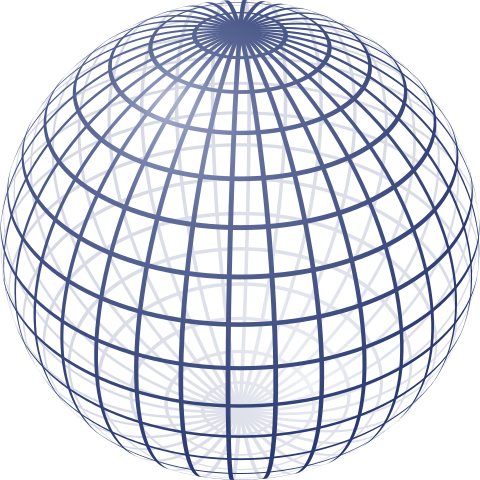
\includegraphics[width=0.3\textwidth]{img/sphere-png.png} 
%\captionsetup{justification=centering}
\caption{Sphere \cite{Spherewi43:online}}
\label{fig:sphere}
%license: attribution 3.0
\end{figure}

Figure \ref{fig:sphere} shows a spherical grid, included here to facilitate visualization of the proposed acoustic system. Consider a speaker at each intersection between two lines and a listener with \textit{in-ear} microphones in the center of the sphere. The acoustic sampling of the sphere, in the \textit{binaural} sense, will take place by sending an ESS from each speaker resulting in two IRs (one for each ear). This complete set of HRIRs, ideally taken in free-field conditions, such as inside an anechoic chamber, contain: time, level, and spectral differences, used by our auditory system to localize sound. \cite{zotkin2006fast} also showed it is possible to invert the microphone and speaker positions to more quickly capture HRTF sets. In their experiment a micro-speaker was placed at the subject's ear canal who was surrounded by a grid of microphones. The benefit of this method is one can capture all the impulse responses for the left ear at once, using a single ESS, then repeat the process for the right ear. Traditionally, HRTF measurements are extremely time consuming which makes personalized HRTFs impractical for most people.

Individual acoustic characteristics the HRIRs have been assigned specific names. \textit{Inter-aural level difference} (ILD) refers to the overall energy difference between the two IRs, \textit{inter-aural time difference} (ITD) refers to the time offset, or phase delay, between measurements. Based on the \textit{diffraction} and \textit{reflection} effects caused by the geometry of the human head, the HRIRs will also exhibit spectral differences, which can be used to discern directions in situations when ITDs and ILDs are not sufficient. Diffraction refers to sounds ability to bend around objects. This is especially true for low frequencies. Reflection refers to sounds ability to bounce off objects. This is especially true for high frequencies.

ILDs are typically caused by the \textit{shadowing effect} of the head and are therefore frequency dependent (\cite{cuevas20193d}). In other words, the ILD will be greater for higher frequencies since lower frequencies diffract, or bend, around the head - while high-frequencies reflect off the head. ITDs are a prominent localization cue at low frequencies and ILDs are the prominent localization cue for mid and high frequency. This concept is known as the \textit{Duplex Theory of Localization} and was proposed by Lord Rayleigh in 1907. 

\subsection{Localization Errors}

Many terms have been defined in the psyscho-acoustic community to describe common localization errors in auditory experiments. Our ability to localize sounds is greatly dependent on the nature of the acoustic environment, as well as the frequency content of the sound source. Also, we should remember that, in the real world, more often than not, multiple sound sources will be present at the same time - making localization tasks even more difficult.

\begin{figure}[ht!]%force figure here, top, strict
\centering
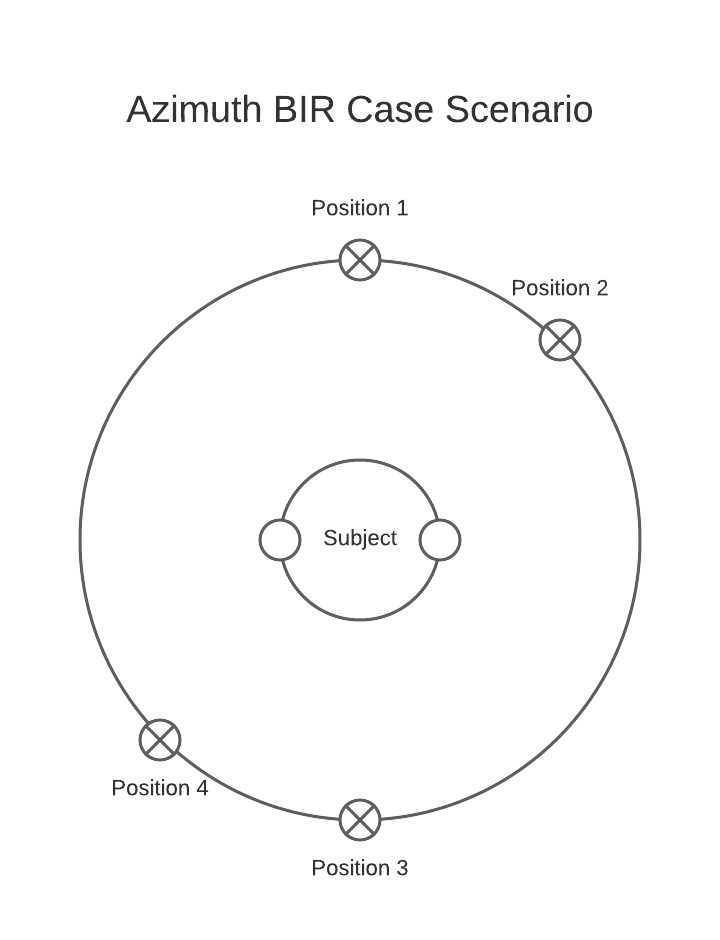
\includegraphics[width=0.5\textwidth]{img/azimuth-bir.png}
%\captionsetup{justification=centering}
\caption{Azimuth BIR Case Scenario}
\label{fig:azimuth-bir}
\end{figure}

In order to demonstrate some common localization errors, we present figure \ref{fig:azimuth-bir}. Consider positions 1 and 3 the figure. Clearly these two positions on the \textit{transverse} plane, otherwise known as the horizontal plane, have identical ILDs and ITDs since the distance from both positions to the subject's ears is identical. Therefore, the subject will only be able to rely on spectral differences to localize the impinging sound. Our outer ear, or \textit{pinna}\footnote{Also called the auricle in some medical textbooks.}, blocks high frequencies arriving from behind the listener, and acts as low-pass filters. The HRIRs capture all these time and frequency differences in order to simulate directionally-dependent sound propagation via \textit{convolution} of the associated IRs; convolution being equivalent to filtering for LTI systems.

In contrast, differentiating between positions 2 and 4 should be substantially easier, since we see that the ITD and ILD differences will compliment spectral differences giving us additional information. Assuming the subject is facing position 1, the distance between position 2 and the subjects right ear, the \textit{ipsilateral} ear\footnote{The ear closest to the source.}, will be smaller than the distance to the \textit{contralateral} ear\footnote{The ear furthest away from the source.}. Sound propagates in air at a rate of around 343 m/s and as it travels it loses energy due to friction between molecules according the \textit{inverse-square law}\footnote{The inverse square law states that with every doubling of distance away from the sound source, the sound will be four times less intense.}. 

\begin{figure}[ht!]%force figure here, top, strict
\centering
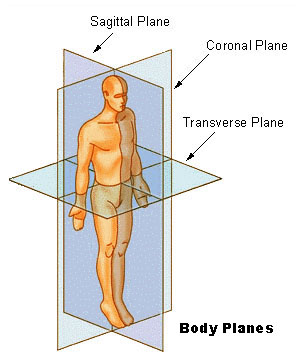
\includegraphics[width=0.5\textwidth]{img/body-planes.jpg}
%\captionsetup{justification=centering}
\caption{Body Planes \cite{body_planes_pic}}
\label{fig:body-planes}
\end{figure}

This additional distance results in a time delay between IRs, as well as level differences. However small these differences might seem, they are crucial for discerning the position of sounds in space. The inability of listeners to differentiate between two sources with identical ITDs and ILDs, when two sources are mirrored over the coronal plane\footnote{Also called the frontal plane.}; is called \textit{front-back confusion}. The same principle applies to sources mirrored over the \textit{transverse plane}\footnote{Also called the horizontal plane.}, these errors are called \textit{up-down confusions}. Sources mirrored over the \textit{mid-sagittal}\footnote{Also known as the longitudinal or median plane.} should be easily discerned since ILDs and ITDs will be quite large. The human auditory system has been shown to be extremely sensitive. The ITD for a typical human head can vary between $\pm$750$\mu$s. Humans can detect ITDs as low as 10-20$\mu$s which correspond to about 1\textdegree in the horizontal plane (\cite{hacihabiboglu2017perceptual}). 

\begin{figure}[ht!]%force figure here, top, strict
\centering
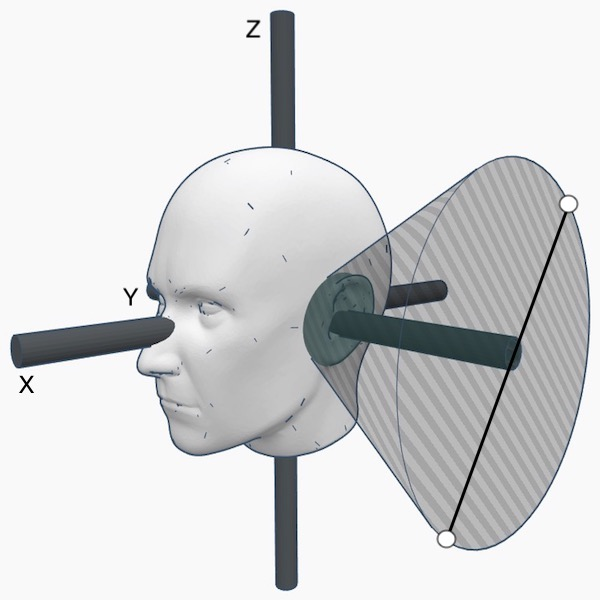
\includegraphics[width=0.5\textwidth]{img/cone_confusion.JPG}
%\captionsetup{justification=centering}
\caption{Cone of Confusion}
\label{fig:cone-confusion}
\end{figure}

The \textit{cone of confusion} is another term used to describe a common phenomenon experienced in localization experiments. Consider the two white dots on the circumference of the cone depicted in figure \ref{fig:cone-confusion}. The two positions, much like any two dots directly opposite each other on this circle, will have identical ITDs and ILDs because their respective distances to the \textit{contralateral} and \textit{ipsilateral} ears, will be the same. In this cases, spectral differences become critical to differentiate between sources. When ambiguous localization tasks arise, small head movements often help resolve source positions.

Our ability to localize sources is most accurate in the horizontal plane. Psycho-acoustic experiments have revealed that \textit{localization blur}, the inability for listeners to discern the direction of a sound, is generally less than 10\textdegree for horizontal sources, but around 20\textdegree for sources in the median plane (\cite{hacihabiboglu2017perceptual}). Two associated objective measures are the \textit{Minimum Audible Angle} (MAA) and the \textit{Minumum Audible Movement Angle} (MAMA). The MAA, a formal term used to quantify \textit{localization blur}, is the minimum detectable angular difference of two successive sound sources \cite{reardon2017evaluation}. The MAMA, is the smallest arc that a moving source must travel to be discriminable from a stationary source \cite{moore1995hearing}.

\subsection{Perception of Distance}

Perception of distance is more complex in some ways than that of orientation. \cite{zahorik2005auditory} provides, a comprehensive overview of auditory distance perception research, including some cognitive science research which examines brain response to acoustic stimuli. As aforementioned, there are several cues that affect our perception of distance - the most salient one being overall energy. A few other unmentioned cues, however, also affect our perception of distance. Among these is the absence or presence of high frequency content in a signal. High frequency signals tend to dissipate faster in air than low frequency ones, because of the additional friction between molecules inherent to these acoustic events. 

\textit{Auditory parallax}, the effect whereby the position or direction of an object appears to differ when heard from different positions, has also been shown to improve distance estimations. Finally, as mentioned before, familiarity tends to affect our perception of sound origin. A sample of a whispering voice, virtually placed far away, will appear closer than it really is. Adversely, a shouting voice, placed close, will appear to be further away than reality. It should be noted that this parallax is not limited to the subjects directional or rotational motion, the movement of the sound source can also help inform our perception of distance.

Finally, \textit{interaural coherence} (IC), the measured statistical coherence of signals received at each ear, aids in distance estimation. In a \textit{diffuse field}, IC is low, because the scattering of sounds off walls interact in unpredictable ways, which result in some amount of randomness in the signals when compared to each other (binaraurally speaking). Therefore, IC can be used as a statistical estimate of distance, since we can assume that in most real-world conditions, sound sources will be diffused acoustically - lowering the overall IC for distant sources more than those proximal.

\subsection{Precedence Effect}

\textit{Summing localization} is a phenomenon - based on ITDs - which affects of perceived direction-of-arrival of sounds. When a broadband signal - a signal with broad range of frequencies present - is played from two directions, with a delay of less than 1 ms, a single event is perceived at the direction between sources. The perceived location shifts towards the first played source, as the delay increases. This \textit{fusion} is one of three characteristics of the \textit{precedence effect}, also known as the \textit{Law of First Wavefront} or \textit{Haas effect}, described in 1949 by Helmut Haas. 

When the delay is between 1 and 5ms, a single event close to the leading source can be heard \cite{hacihabiboglu2017perceptual}. The lagging source - the delayed copy of the sound - can be perceived due to the change in timbre, and is perceptually equivalent to a feedforward comb filter where the delayed copy is played back over a second discrete channel. In this context, the \textit{echo threshold}, refers to the amount of delay that must be introduced to the copy before we begin perceiving the two sounds as independent non-fused events. This threshold is dependent on the nature of the signal. For a short broadband click, 5 ms might be enough to create an echo. For music and speech signals, the threshold is longer, and can be as high as 20 ms.

The precedence effect can be summarized by the following three phenomena: 

\todo[inline]{Each time I make a list I make the terms bold. I should make this standard throughout. Find "enumerate".}

\begin{enumerate}
    \item \textbf{Localization dominance}: the direction of an auditory event depends predominantly on the leading source.
    \item \textbf{Fusion}: a single auditory event is perceived when two sound events are below the \textit{echo threshold}.
    \item \textbf{Lag Discrimination Suppression}: the direction of the lagging sound is suppressed.  
\end{enumerate}

\subsection{Doppler Shift}

\textit{Doppler shift} is another auditory cue, related to \textit{auditory parallax}, which can aid in our estimation of source distance and direction. Doppler shift is the phenomenon we experience when we perceive the pitch of an ambulance's siren, or any other moving source, change as it approaches or moves away from us. Specifically, as the ambulance siren moves towards us, the pitch seems be higher than when stationary, and as it moves away, it seems to be lower than when stationary. This has to do with the nature of longitudinal waves, which contract and expand in relation to the speed of the object. \cite{lavalle2016virtual} provides a whole chapter on the auditory mechanisms involved in Virtual Reality (VR). The book also covers the fundamentals of VR optics, interaction, and tracking, and is recommended for anybody interested in Extended Reality (XR). Equation \ref{eq:doppler}, from chapter 11, describes our perceived frequency of sound as a function of it's velocity. By combining this auditory cue with distance based intensity dampening we can realistically simulate moving sources.

\begin{equation}
f_{r}=\left(\frac{s+v_{r}}{s+v_{s}}\right) f_{s}
\label{eq:doppler}
\end{equation}

Where: 
\begin{description}
    \item $f_r$ is the resulting frequency.
    \item $s$ is the speed of sound (343.2 m/s roughly at C 20\textdegree).
    \item $v_r$ is the velocity of the receiver (negative if receiver is moving away). 
    \item $v_s$ is the velocity of the source (negative is the source is moving away).
    \item $f_s$ is the original frequency of the source.
\end{description}
    
\subsection{Binaural Synthesis Errors}

Of particular importance to our work is the use of binaural synthesis for the simulation of acoustic spaces. Binaural synthesis allows us to experiment with \textit{spatial music} without the need for sophisticated and often inaccessible loudspeaker systems. In binaural synthesis, sound sources are dynamically \textit{convolved}\footnote{As noted, convolution of a source with an impulse response is equivalent to applying a filter in LTI theory.} with HRIRs to simulate surround sound experiences. Binaural synthesis has become increasingly popular with the growth of \textit{extended reality} (XR) systems. However, several problems, such as: non-personalized HRTFs, externalization errors, and localization issues; persist. 

% \todo[inline]{talk about non-personalized HRTFs and localization errors. }

Personalized HRTFs are believed to be part of the key to solving front-back confusions sometimes experienced in binaural synthesis \cite{johansson2019vr}. Unfortunately, these tend to be too laborious for most people. An additional problem was the lack of a standardized format for sharing HRTF data. Recently the Spatially Oriented Format for Acoustics (SOFA) format was designed to alleviate this issue \cite{majdak2013spatially}. Johansson \cite{johansson2019vr} also notes two additional problems with binaural synthesis that warrant more exploration:

\begin{enumerate}
    \item Coloration artefacts which might be the result of poor HRTF measurement techniques. Another theory is that personalized HRTFs offer less coloration of the frequency spectrum.
    \item The lack of "dynamic HRTFs", which he describes as those that model head movement independently of shoulder movements. 
\end{enumerate}

Poor \textit{externalization}\footnote{Also sometimes referred to as Inside-the-Head Locatedness (IHL).}, the degree to which listeners perceive sources as originating inside their head, can be mitigated by the use of a head-tracking system. The systems, based on \textit{inertial measurement units} (IMU), monitor the orientation of the listener's head and adjusts the soundfield accordingly. When no rotation adjustment is included, our auditory system assumes that sources must be originating from inside our head, as this is the only rational conclusion for sources without dynamic filtering based on BIRs. The subtle spectral changes from location to location, provided by head-tracking, provide a way to disambiguate between source positions. The addition of diffuse field modeling, in the form of reverberation unit, also supports improved \textit{externalization}(\cite{sakamoto1976out}). 

\subsection{Reverberation}
%Room acoustics. T60, etc. Sabine equation. RT60. 

An important element of spatialization in virtual auditory environments (VAE) or in real-world environments is the reverberant characteristics of a space. Reverberation occurs when a dense network of echoes, with sufficiently small delay, mesh together to form a cohesive spatial image\footnote{The term spatial image used here to denote how the sound informs our perception of space.}. Sometimes the reverberation can be considered an obtrusive feature of a space, which reduces the intelligibility of the a signal. Other times, it can be deemed desirable, such as when musical events with harmonic relationships are performed in the reverberant space, this creating pleasing textures. 

Reverberation can provide the impression of realism, as sounds in space are seldom devoid of reverberation. It can also be pushed beyond the real towards artistic goals. Control over different characteristics of reverberation can be accomplished both in the architectural and digital domain. Since artists rarely have any control of architectural acoustics, and since this document is more closely concerned with computer-music approaches to spatialization, we will cover reverb processors from a software perspective. Some of the same principles, however, can be applied to architectural treatment of spaces. We refer the reader to \cite{gupta2019analysis} for a brief and concise overview of room acoustic design for recording studios. Finally, \cite{beranek1992concert} provides an overview of concert hall acoustics. 

\todo[inline]{I will come back to write this section. There is a lot to cover. I think I will skip most reverb designs and focus only on multi-channel ones. I will give a reference for stereo reverb designs.}

% \subsubsection{Algorithmic Reverbs}
% \subsubsection{Convolution Reverbs}

\section{Conclusion}
This concludes our introduction to the subject of spatial sound. In this chapter we have presented the reader with different perspectives from which to begin appreciating the complexity of the field, and some background knowledge which should provide clarity to the proceeding chapters. Namely, we touched briefly on the compositional, psycho-acoustic and some of the engineering aspects of this domain. The next chapter will talk more in depth about the artistic practice of spatial sound drawing on historically important musical works, particularly in the field of electro-acoustic music. Chapter \ref{ch:spat-mus} will also talk about the development of spatial instruments which facilitate the creation of these works, and are sometimes indispensable to the recreation of these pieces.